\documentclass[a4paper,11pt]{article}
\usepackage[utf8]{inputenc}
\usepackage{amsmath, amssymb, amsthm}
\usepackage{graphicx}
\usepackage{hyperref}
\usepackage{geometry}
\geometry{margin=1in}

\title{Estimation of Schatten $p$-Norms of Large Matrices \\ using Krylov Subspace Methods}
\author{Martin}
\date{\today}

\begin{document}

\maketitle

\begin{abstract}
The exact computation of Schatten $p$-norms for large-scale matrices poses a significant computational challenge due to the $\mathcal{O}(N^3)$ complexity of the Singular Value Decomposition (SVD). In this report, we discuss mathematical foundations and efficient algorithmic strategies to estimate these norms. By employing stochastic trace estimators combined with Krylov subspace methods, we reduce the computational footprint to $\mathcal{O}(N)$. We provide theoretical background on the underlying matrix functions and describe the Stochastic Lanczos Quadrature (SLQ) and Golub-Kahan Bidiagonalization (GKB) methods. Preliminary numerical results and performance plots are also presented.
\end{abstract}

\section{Introduction}

The Schatten $p$-norm of a matrix $A \in \mathbb{C}^{N \times N}$ is defined as the $\ell_p$-norm of its singular values. Let $\sigma_1, \sigma_2, \dots, \sigma_N$ be the singular values of $A$. The Schatten $p$-norm is given by:
\begin{equation}
    \|A\|_p = \left( \sum_{i=1}^N \sigma_i^p \right)^{1/p}.
\end{equation}
For $p=1$, this corresponds to the nuclear norm; for $p=2$, the Frobenius norm; and as $p \to \infty$, it converges to the spectral norm (the largest singular value). 
Evaluating $\|A\|_p$ exactly requires full knowledge of the singular spectrum, which is typically acquired via the SVD. For large dimensions, this approach is computationally prohibitive both in time and memory. Therefore, we utilize advanced numerical linear algebra techniques, specifically randomized trace estimators and Krylov subspace methods, to approximate these norms efficiently \cite{benzi2023computation, arrigo2016computation}.

\section{Theoretical Background}

\subsection{Matrix Functions and Trace Estimation}

The Schatten $p$-norm can be reformulated as the trace of a specific matrix function. Since the singular values of $A$ are the square roots of the eigenvalues of the Hermitian positive semi-definite matrix $A^\dagger A$, we can write:
\begin{equation}
    \|A\|_p^p = \sum_{i=1}^N \sigma_i^p = \mathrm{tr}\left( (A^\dagger A)^{p/2} \right).
\end{equation}
Thus, estimating the Schatten $p$-norm is mathematically equivalent to estimating the trace of the matrix function $f(A^\dagger A) = (A^\dagger A)^{p/2}$. 

Evaluating the trace of a large implicit matrix can be effectively handled using Hutchinson's stochastic trace estimator. For a symmetric or Hermitian matrix $B$, Hutchinson's estimator approximates the trace as:
\begin{equation}
    \mathrm{tr}(B) \approx \frac{1}{s} \sum_{i=1}^s x_i^\dagger B x_i,
\end{equation}
where $x_1, \dots, x_s$ are random vectors with independent identically distributed entries satisfying $\mathbb{E}[x_i x_i^\dagger] = I$. Typically, Gaussian or Rademacher (random signs) distributions are employed. This reduces the trace computation to evaluating bilinear forms $x_i^\dagger f(A^\dagger A) x_i$ \cite{benzi2026estimation}.

\subsection{Krylov Subspace Methods}

The remaining challenge is to evaluate the bilinear form $x^\dagger f(A^\dagger A) x$ without explicitly computing $A^\dagger A$ or its full spectrum. To this end, Krylov subspace methods are uniquely powerful \cite{saad2003iterative}.

Given a matrix $M = A^\dagger A$ and a starting vector $x$, the $m$-th Krylov subspace is defined as:
\begin{equation}
    \mathcal{K}_m(M, x) = \mathrm{span}\{x, M x, M^2 x, \dots, M^{m-1} x\}.
\end{equation}
Krylov methods project the high-dimensional operator $M$ onto the low-dimensional subspace $\mathcal{K}_m(M, x)$, constructing an orthonormal basis $V_m \in \mathbb{C}^{N \times m}$ and a small projection matrix $T_m = V_m^\dagger M V_m$, which is tridiagonal in the Hermitian case. 

The application of the matrix function to the vector $x$ can then be approximated by evaluating the function on the much smaller matrix $T_m$:
\begin{equation}
    f(M)x \approx \|x\|_2 V_m f(T_m) e_1,
\end{equation}
which immediately yields the scalar approximation $x^\dagger f(M) x \approx \|x\|_2^2 e_1^T f(T_m) e_1$. This approximation is formally equivalent to Gaussian quadrature rules with respect to the spectral measure of $M$ at the starting vector $x$ \cite{benzi2023computation, arrigo2016computation}.

\section{Algorithmic Approaches}

\subsection{Stochastic Lanczos Quadrature (SLQ)}

The SLQ algorithm directly leverages the symmetric Lanczos process on $M = A^\dagger A$. 
For each random starting vector $x_i$:
\begin{enumerate}
    \item Run the Lanczos algorithm on $A^\dagger A$ for $m$ iterations to build the tridiagonal matrix $T_m$.
    \item Compute the eigendecomposition of the $m \times m$ matrix $T_m = U D U^T$.
    \item Approximate the quadratic form as $x_i^\dagger (A^\dagger A)^{p/2} x_i \approx \|x_i\|_2^2 \sum_{k=1}^m [U]_{1,k}^2 D_{k,k}^{p/2}$.
\end{enumerate}
SLQ requires the application of $A$ and $A^\dagger$ at every step, meaning it only needs matrix-vector products, keeping memory bounded at $\mathcal{O}(N)$ instead of $\mathcal{O}(N^2)$.

\subsection{Golub-Kahan Bidiagonalization (GKB)}

Instead of applying Lanczos directly to $A^\dagger A$, which squares the condition number, the Golub-Kahan Bidiagonalization process operates on $A$ directly. The GKB process iteratively builds orthogonal bases $U_\ell \in \mathbb{C}^{N \times \ell}$ and $V_\ell \in \mathbb{C}^{N \times \ell}$ such that:
\begin{equation}
    A V_\ell = U_\ell B_\ell, \quad A^\dagger U_\ell = V_\ell B_\ell^\dagger + \gamma_\ell v_{\ell+1} e_\ell^T,
\end{equation}
where $B_\ell$ is a lower bidiagonal matrix. The tridiagonal matrix generated by applying Lanczos to $A^\dagger A$ is algebraically equivalent to $T_\ell = B_\ell^\dagger B_\ell$. We then evaluate the matrix function on the small bidiagonal matrix $B_\ell$ to approximate the trace \cite{arrigo2016computation}.

\section{Preliminary Results}

To empirically analyze the implemented methods, we tested the scalability of the algorithms using Kronecker tensor powers of a $3\times3$ random density matrix: $\rho^{\otimes n}$. This allowed us to organically scale the matrix dimension $N = 3^n$.

\begin{figure}[h!]
    \centering
    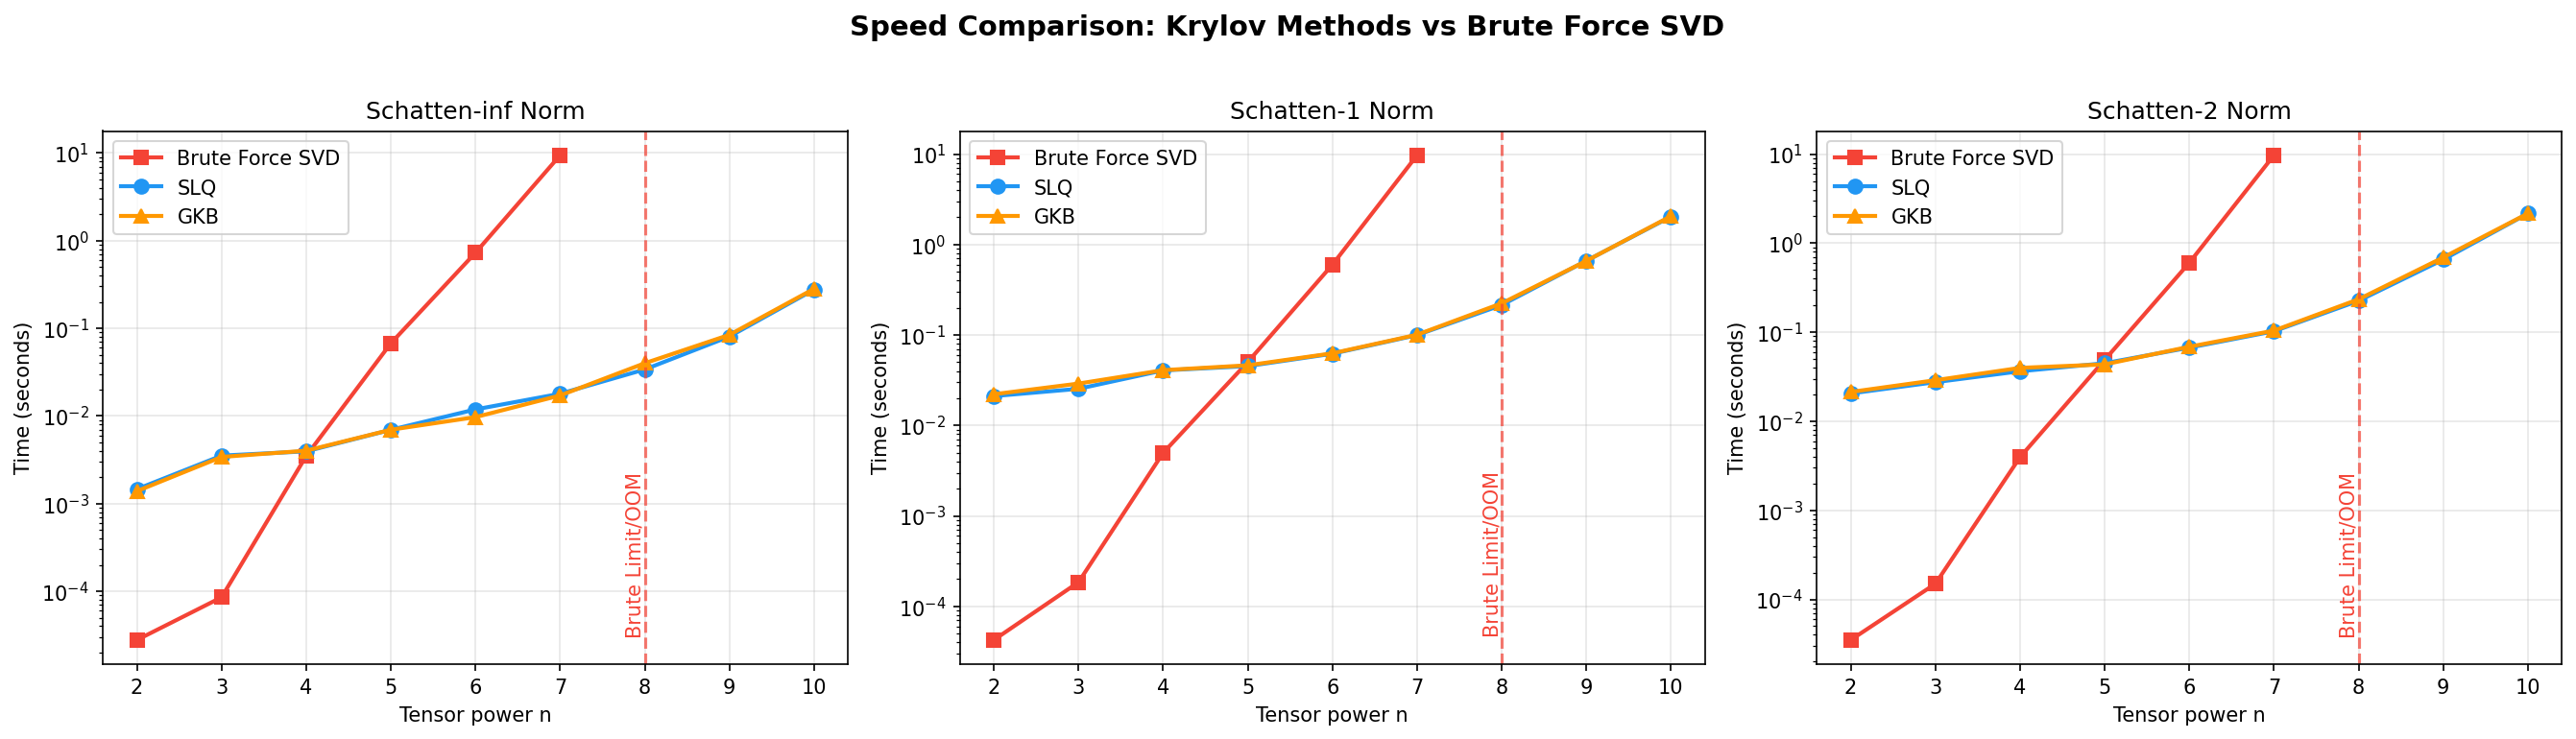
\includegraphics[width=0.8\textwidth]{speed_comparison.png}
    \caption{Speed comparison of Brute Force SVD versus Krylov-based SLQ and GKB estimators over increasing tensor powers $n$.}
    \label{fig:speed}
\end{figure}

\begin{figure}[h!]
    \centering
    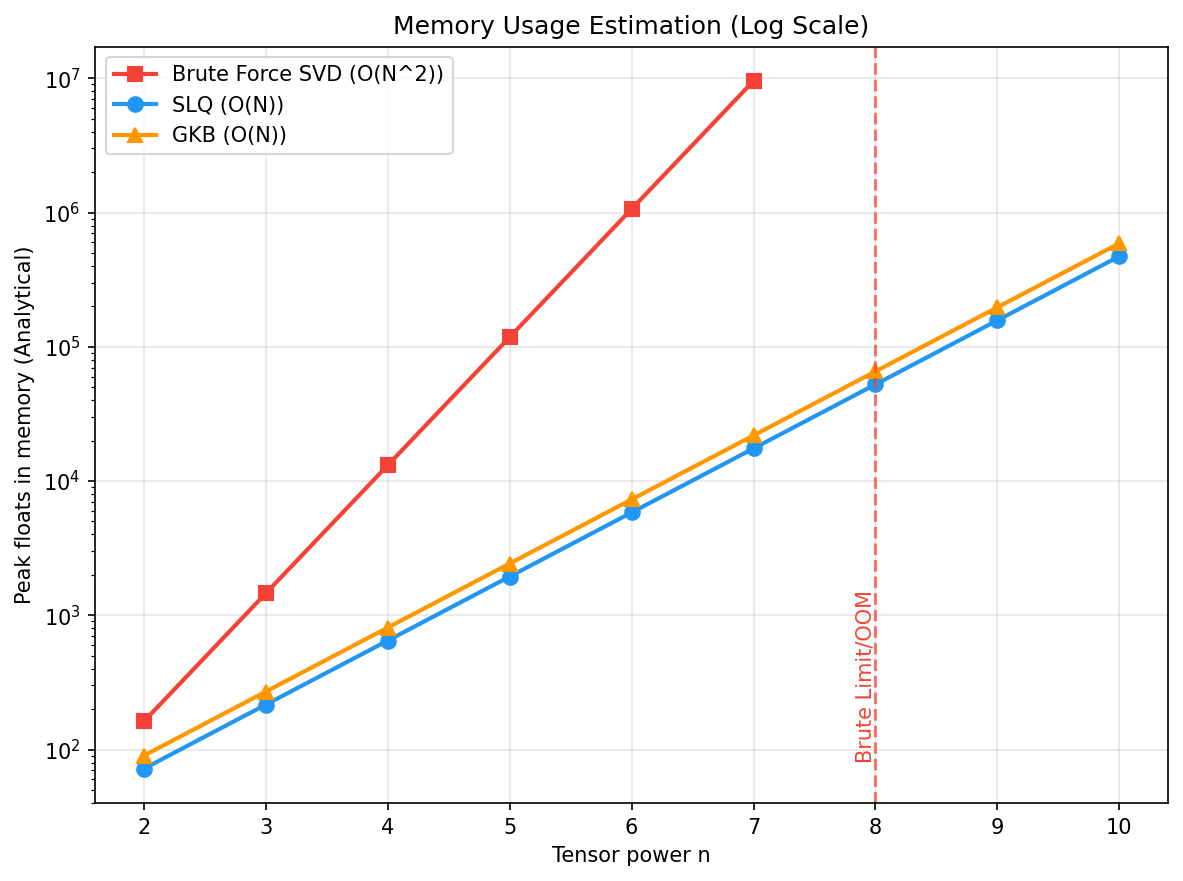
\includegraphics[width=0.8\textwidth]{memory_comparison.png}
    \caption{Peak memory consumption analysis highlighting the theoretical linear scaling of Krylov methods compared to the quadratic cost of exact SVD.}
    \label{fig:memory}
\end{figure}

As shown in Figure \ref{fig:speed} and Figure \ref{fig:memory}, the $\mathcal{O}(N^3)$ computational time and $\mathcal{O}(N^2)$ spatial constraints of the exact Brute Force SVD make it intractable beyond $n=8$ (causing Out Of Memory, or OOM, failures). Conversely, SLQ and GKB easily bypass this bottleneck due to their matrix-free $\mathcal{O}(N)$ architecture. A massive, comprehensive run over larger parameter spaces and complex graphs is scheduled for future exploration.

\section{Future Work}
In upcoming iterations, we intend to execute exhaustive large-scale experiments to determine the tightest bounds on error oscillations and assess robust stopping criteria (including consecutive difference estimations) for arbitrary non-Hermitian graphs and density matrices.

\bibliographystyle{plain}
\bibliography{citation}

\end{document}
